\documentclass[11pt, a4paper]{article}
\usepackage[UKenglish]{babel}
\usepackage[bibstyle=ieee, dashed=false, sorting=nty]{biblatex}
\usepackage[labelfont=bf]{caption}
\usepackage{csquotes}
\usepackage{fancyhdr}
\usepackage{float}
\usepackage{graphicx}
\usepackage[top=25mm, right=20mm, bottom=25mm, left=20mm]{geometry}
\usepackage[hidelinks]{hyperref}
\usepackage{microtype}
\usepackage{parskip}
\usepackage[small,compact]{titlesec}

\titlespacing*{\section}{0pt}{\baselineskip}{0.35\baselineskip}

\pagestyle{fancy}
\fancyhf{}
\fancyhead[L]{COM3504}
\fancyhead[C]{The Intelligent Web: Assignment}
\fancyhead[R]{Team: Gakki}
\fancyfoot[C]{\thepage}

\addbibresource{references.bib}

\begin{document}
\section{Introduction}
Progressive Web App (PWA) allows users to create and add comments to both events and user stories.
Social media features such as `like', `follow', `interested', and `going' were integrated. Users are
able to tag an event with their stories, which will then appear in the `Explore' page. Users can
create a story by taking a picture with their front camera through the use of
of WebRTC or upload a picture locally. Each user story can receive likes and comments, for which
the latter was implemented using Socket.IO \cite{week6, socketio}. Service worker was implemented
to cache requests for offline usage. MongoDB is used to store and synchronise data between the
client and server, while IndexedDB is used to store data loaded from MongoDB for offline usage.
However, data stored in MongoDB can only be retrieved when user is online. The search function (via
location) was implemented with Google Maps API, allowing auto complete for the location field and
ensuring that it is a valid location. For security purposes, users can only login with their
respective Google Account.

\section{Diagrams}
Appendix \hyperref[figure:site_map]{\textbf{Figure 1}} and Appendix \hyperref[figure:uml]{
\textbf{Figure 2}} are the detailed description of the PWA system structure with
\hyperref[figure:site_map]{\textbf{Figure 1}} describing the interactions between the front-end,
data storage, caching and data retrieval, while \hyperref[figure:uml]{\textbf{Figure 2}}
demonstrates the database model along with the relationship between documents.

\section{Interface to Insert and Search Data via Forms}
\textbf{Challenges:} Search speed must be efficient and search results must be
accurate with respect to the given query. Users must be able to search for events, stories, and
profile of other users. Basic text search will allow the user to input any text query and return the
results sorted by relevance. Users can use partial words to search for an event or profiles of other
users. Advanced search will allow the user to search for events based on event name, venue (address)
and date. When creating an event, Place Autocomplete by Google Maps API \cite{google_maps_api} is
used to provide users with valid locations as options. \textbf{Solution:} FlexSearch.js
\cite{flexsearch} was chosen to implement basic text searching task due to its efficient,
lightweight, and flexible properties \cite{flexsearch_benchmarkk}. It allows multi-field search and
accepts multiple data format types as data index. Hence, it is used with both MongoDB and IndexedDB
to provide searching functionality in both online and offline environment respectively.
\textbf{Requirements:} Users should be able to search for events and user profiles while online and
offline. Users should be able to obtain results through querying with partial information. The
results returned are sorted by relevance. \textbf{Limitations:} On every page load, the data has to
be retrieved from IndexedDB to populate the FlexSearch.js's search index. The performance loss might
be negligible when the total data size is small, but it may cause longer loading time when the size
of data exceeds a certain size. Google Maps API request could not be cached as it generates a random
token for every request made, hence Place Autocomplete will not work offline.

\section{Interface to Search Data via Map}
\textbf{Challenges:} Allow users to search and locate ongoing or upcoming events via map, where
marker containing the image and link to event is placed on the location of the event.
\textbf{Solutions:} Map was implemented with Leaflet Geocoder, with markers displaying pop-up of
image and link of ongoing and future events. Offline searches will display marker on cached location
of event. \textbf{Requirements:} Allow users to search for events using a map in both online and
offline environments. Past events should not appear on the map. Future and ongoing events should be
displayed as custom markers on the map. Custom markers should pop-up to display the event
information when clicked. \textbf{Limitations:} The map takes time to load and does not generate
immediately. Google Maps API was not chosen to be implemented in this task as request could not be
cached due to the generation of random token for every request made, making it unavailable when user
is offline. Caching the map tiles consumes more storage than other requests as map tiles are stored
as images. If Place Autocomplete by Google Maps API \cite{google_maps_api} was not implemented,
users would be able to insert invalid locations, causing markers of any previously created events
with valid locations to not show up on the map. Hence, heavily relies on the input to be of valid
locations.

\section{PWA – Caching of the App Template Using a Web Worker}
\textbf{Challenges:} Fetching cross-domain response will result in an opaque response, which will
consume huge storage quota compared to normal responses \cite{opaque_workbox}. Sending a fallback
offline page response when user is offline and visit a page that does not exist in the cache.
\textbf{Solutions:} `Cache then network' was used and modified according to The Offline Cookbook
\cite{offline_cookbook}. \textbf{Requirements:} Users should be able to view a basic offline
template with required data when page was not visited in the past and user is offline. Users should
be able to view previously loaded events, stories, and profiles without the ability to make any
changes. \textbf{Limitations:} Non-static files are not cached in the installation stage
of the service worker. Page that has never been visited before will not be cached. This applies to
events or stories which were updated, where instead of the updated information, the cached
information, which might not be up-to-date, will be displayed when user is offline.

\section{PWA: Caching Data Using IndexedDB}
\textbf{Challenges:} Retrieve data from MongoDB and store them in IndexedDB. Display page content
using data loaded from IndexedDB when no internet connection is present. \textbf{Solution:} Retrieve
data from MongoDB using AJAX. Promise is used for both storing and loading of data from IndexedDB.
\textbf{Requirements:} Data on events and user profiles must be stored locally for offline searching.
Users should be able to access data retrieved from IndexedDB when they are offline.
\textbf{Limitations:} A known bug of IndexedDB storage is usage increases with every $put()$
operation \cite{leveldb_593, leveldb_603}.

\section{NodeJS Server Including Non-Blocking Organisation of Multiple Dedicated Servers}
\textbf{Challenges:} Uses asynchronous functions to handle file upload, data retrieval from server,
or other function calls that require time to complete. Errors might occurred during the execution
of asynchronous functions. \textbf{Solution:} Uses the Promise and async/await features of
JavaScript to handle both successful and failed function operations. Keep the code nesting shallow
to make code more maintainable and readable. \textbf{Requirements:} Able to use Promise to order the
sequence of asynchronous processes. Able to use callbacks to handle the success and failure of
asynchronous functions. \textbf{Limitations:} Single threaded mechanism, not suitable for
CPU-intensive operations. Relies heavily on callbacks, which might possibly result in several
callbacks nested within order callbacks.

\section{MongoDB}
\textbf{Challenges:} Creating schemas that clearly define the respective models. Verifying user
inputs when creating a new document. \textbf{Solution:} Uses mongoose's validation middleware
\cite{validation} to define the values allowed for an index. \textbf{Requirements:} Data stored in
MongoDB must be synchronised with IndexedDB when the client has connection to the server.
\textbf{Limitations:} Lacks flexibility as it does not support joins between multiple documents.
Document size has a limit of 16MB, additional configurations were required for storing large images.

\section{Quality of the Web Solution}
\textbf{Challenges:} Implementation of an authentication system. Researching and implementing social
features such as user profile, marking events as `Interested' or `Going'. Ensuring that the features
implemented will work and do not cause system failure. \textbf{Solution:} Used
passport-google-oauth20 \cite{passport_google} to implement the authentication system. AJAX
requests are used for a non-page reload form submission. Exhaustively testing the system to
minimise the probability of bug occurrences. \textbf{Requirements:} Users should be able to select
events to be tagged to their stories, 'like' and comment on stories, 'follow' other users, and click
`Interested' or `Going' on events. Events which users attended are recorded in their profile. Events
which were created by a user is set to be an event the organiser is `Going' to by default. Through
following others and posting themselves, users are able to view the activity of followed users and
their own post, be it events or stories, in the `Home' page. Users require a Google Account to login
for security purposes. In the implementation of WebRTC, a range of filters were made available for
users to choose from. Another extra feature is in the implementation of map search where users are
not just able to view the event name but also a link which would lead the user to the page
displaying details of that specific event. Having Google Maps API Place Autocomplete also helps
users to quickly and accurately insert a valid location. Users are also able to list their favourite
genres and write a bios to guide other users in finding those of similar interest, and possibly
follow them. This in done to increase users' experience to have information of interest displayed
on their `Home' page upon login. \textbf{Limitations:} Users without a Google Account could not
sign in into the system and enjoy personalised functionalities. Users who are not signed-in are
able to view events, stories, and use the search functionalities, but are unable to show their
interest through clicking on `Interested' or `Going', which would be displayed in their profiles.
They would not be able to update any information, follow or unfollow other users, or like and
comment on stories. As mentioned above, Google Maps API do not work offline. However, this is a
minor limitation here since users are not able to make changes when they are offline. User accounts
are all public, hence users should be careful when sharing personal information.

\section{Conclusions}
This assignment highlights the importance of caching and the importance of usability both during
online and offline. It taught us to consider other implementations to improve user experience and
web security. This assignment exposed us to multiple tools (Google Maps API for address searching,
WebRTC for photo capturing, Socket.IO for live comment updates, Leaflet Geocoder for map searching
with markers, etc.) while allowing us to implement the basic knowledge of web building at a higher
level through the use of promises, service workers and memory caching.

\section{Division of Work}
The solution was designed jointly. \textbf{Zer Jun Eng} lead implementation of MongoDB, search
by map, PWA caching, and front-end implementation while taking part in WebRTC, testing.
\textbf{Lim Jia Mei Grace (Jia Lim)} lead implementation of WebRTC, testing, and documentation
while taking part in the construction of MongoDB database, search by map and front-end
implementation. The final document was jointly edited. 

\section{Extra Information}
Run \textbf{npm run initdb} to populate the database with initial data, then run \textbf{npm start}
to start localhost and MongoDB.

\printbibliography

\appendix
\section{Appendix}
\begin{figure}[H]
  \begin{center}
      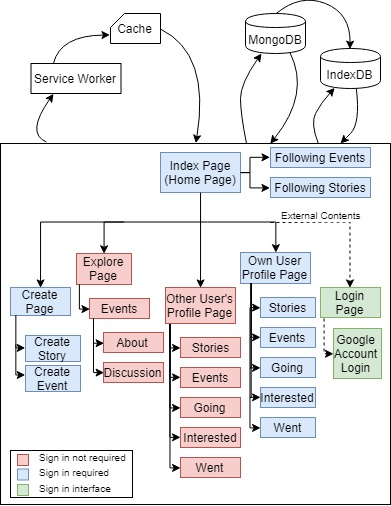
\includegraphics[width=8.7cm]{site_map.jpg}
      \caption{Demonstrates the flow of each web page in this PWA system along with the respective
      partial pages and external content pages.}
      \label{figure:site_map}

      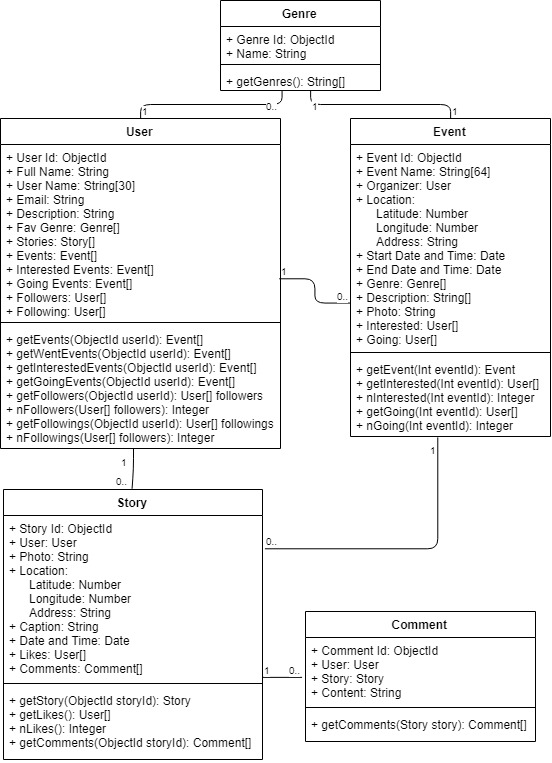
\includegraphics[width=8.7cm]{uml.jpg}
      \caption{Displays the structure of the database along with the types of content stored.}
      \label{figure:uml}
  \end{center}
\end{figure}


\end{document}
